% The reduced transition matrix: where the temporal cut sits in the strip, how it appears in the
% tensor network, and the object left after contracting the two halves.
% Conventions and row structure follow imgs/echo_strip.tex (time upwards, space to the right, cream
% for the cooling rows, open circles for the product state). The split into an open part of height t
% and a traced part of height T-t follows Fig. 2 of carignano_tagliacozzo2025.
%
% Standalone: compiles to imgs/rtm_strip.pdf.
% Inline:     with \usepackage{standalone}, % The reduced transition matrix: where the temporal cut sits in the strip, how it appears in the
% tensor network, and the object left after contracting the two halves.
% Conventions and row structure follow imgs/echo_strip.tex (time upwards, space to the right, cream
% for the cooling rows, open circles for the product state). The split into an open part of height t
% and a traced part of height T-t follows Fig. 2 of carignano_tagliacozzo2025.
%
% Standalone: compiles to imgs/rtm_strip.pdf.
% Inline:     with \usepackage{standalone}, % The reduced transition matrix: where the temporal cut sits in the strip, how it appears in the
% tensor network, and the object left after contracting the two halves.
% Conventions and row structure follow imgs/echo_strip.tex (time upwards, space to the right, cream
% for the cooling rows, open circles for the product state). The split into an open part of height t
% and a traced part of height T-t follows Fig. 2 of carignano_tagliacozzo2025.
%
% Standalone: compiles to imgs/rtm_strip.pdf.
% Inline:     with \usepackage{standalone}, % The reduced transition matrix: where the temporal cut sits in the strip, how it appears in the
% tensor network, and the object left after contracting the two halves.
% Conventions and row structure follow imgs/echo_strip.tex (time upwards, space to the right, cream
% for the cooling rows, open circles for the product state). The split into an open part of height t
% and a traced part of height T-t follows Fig. 2 of carignano_tagliacozzo2025.
%
% Standalone: compiles to imgs/rtm_strip.pdf.
% Inline:     with \usepackage{standalone}, \input{imgs/rtm_strip}.
\documentclass[tikz,border=3pt]{standalone}
\usepackage{amsmath,amssymb,braket}
\usetikzlibrary{arrows.meta,fadings}

\newcommand{\DX}{0.96}
\newcommand{\DY}{0.60}
\newcommand{\TCUT}{3.5}      % height of the cut, in row units

\definecolor{tnbulk}{RGB}{86,196,229}
\definecolor{tncool}{RGB}{240,224,178}

\begin{document}
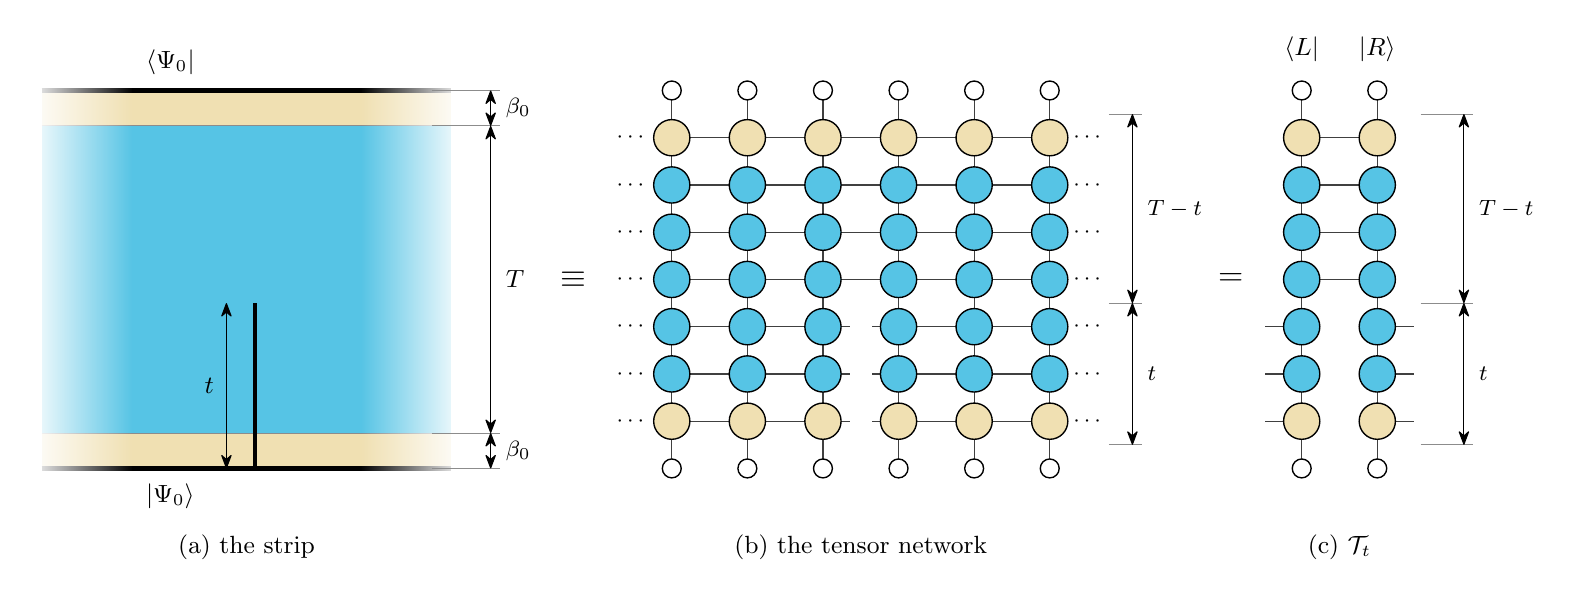
\begin{tikzpicture}[
    >={Stealth[round,length=2.0mm]},
    leg/.style={draw=black!75, line width=0.45pt},
    W/.style={circle, draw=black, fill=tnbulk, line width=0.5pt, minimum size=4.6mm, inner sep=0pt},
    B/.style={circle, draw=black, fill=tncool, line width=0.5pt, minimum size=4.6mm, inner sep=0pt},
    P/.style={circle, draw=black, fill=white, line width=0.5pt, minimum size=2.4mm, inner sep=0pt},
    cutline/.style={draw=black, line width=1.3pt},
    guide/.style={draw=black!45, line width=0.35pt},
    tag/.style={font=\small},
    idx/.style={font=\footnotesize},
  ]

  %% ================= panel (a): the strip, with the cut of height t =================
  \begin{scope}
    \def\SW{5.2}
    \def\YA{0} \def\YB{0.75} \def\YC{7.25} \def\YD{8}

    \fill[tncool] (0,{\YA*\DY}) rectangle (\SW,{\YB*\DY});
    \fill[tnbulk] (0,{\YB*\DY}) rectangle (\SW,{\YC*\DY});
    \fill[tncool] (0,{\YC*\DY}) rectangle (\SW,{\YD*\DY});
    \draw[black, line width=1.6pt] (0,{\YA*\DY}) -- (\SW,{\YA*\DY});
    \draw[black, line width=1.6pt] (0,{\YD*\DY}) -- (\SW,{\YD*\DY});
    \draw[guide] (0,{\YB*\DY}) -- (\SW,{\YB*\DY});
    \draw[guide] (0,{\YC*\DY}) -- (\SW,{\YC*\DY});

    \fill[white, path fading=east] (-0.18,{\YA*\DY-0.12}) rectangle (1.15,{\YD*\DY+0.12});
    \fill[white, path fading=west] ({\SW-1.15},{\YA*\DY-0.12}) rectangle ({\SW+0.18},{\YD*\DY+0.12});

    \node[tag, anchor=north west] at (1.2,{\YA*\DY-0.07}) {$\ket{\Psi_0}$};
    \node[tag, anchor=south west] at (1.2,{\YD*\DY+0.07}) {$\bra{\Psi_0}$};

    % the cut: a solid line from the bottom edge up to height t
    \draw[cutline] ({0.52*\SW},{\YA*\DY}) -- ({0.52*\SW},{\TCUT*\DY});
    \draw[<->] ({0.52*\SW-0.36},{\YA*\DY}) -- ({0.52*\SW-0.36},{\TCUT*\DY})
      node[midway, left=1pt, tag] {$t$};

    \def\XD{\SW+0.5}
    \foreach \y in {\YA,\YB,\YC,\YD} {
      \draw[guide] ({\SW-0.25},{\y*\DY}) -- ({\XD+0.12},{\y*\DY});
    }
    \draw[<->] ({\XD},{\YB*\DY}) -- ({\XD},{\YC*\DY}) node[midway, right=2pt, tag] {$T$};
    \draw[<->] ({\XD},{\YA*\DY}) -- ({\XD},{\YB*\DY}) node[midway, right=2pt, idx] {$\beta_0$};
    \draw[<->] ({\XD},{\YC*\DY}) -- ({\XD},{\YD*\DY}) node[midway, right=2pt, idx] {$\beta_0$};

    \node[tag] at ({\SW/2},-1.0) {(a) the strip};
  \end{scope}

  \node[font=\large] at (6.75,{4*\DY}) {$\equiv$};

  %% ================= panel (b): the tensor network, the cut removes the bonds =========
  \begin{scope}[xshift=8.0cm]
    \def\NX{5}

    \foreach \i in {0,...,\NX} { \draw[leg] (\i*\DX,0) -- (\i*\DX,{8*\DY}); }
    % every horizontal bond except those crossed by the cut
    \foreach \j in {1,...,7} {
      \foreach \i in {0,1,3,4} { \draw[leg] (\i*\DX,\j*\DY) -- ({(\i+1)*\DX},\j*\DY); }
    }
    \foreach \j in {4,...,7} { \draw[leg] ({2*\DX},\j*\DY) -- ({3*\DX},\j*\DY); }
    % below the cut there is no bond: each side keeps an open leg
    \foreach \j in {1,2,3} {
      \draw[leg] ({2*\DX},\j*\DY) -- ({2*\DX+0.34},\j*\DY);
      \draw[leg] ({3*\DX},\j*\DY) -- ({3*\DX-0.34},\j*\DY);
    }

    \foreach \i in {0,...,\NX} {
      \foreach \j in {1,7} { \node[B] at (\i*\DX,\j*\DY) {}; }
      \foreach \j in {2,...,6} { \node[W] at (\i*\DX,\j*\DY) {}; }
      \node[P] at (\i*\DX,0)       {};
      \node[P] at (\i*\DX,{8*\DY}) {};
    }
    \foreach \j in {1,...,7} {
      \node[idx] at (-0.5,\j*\DY)           {$\cdots$};
      \node[idx] at ({\NX*\DX+0.5},\j*\DY)  {$\cdots$};
    }

    % the two parts of the temporal chain
    \def\XB{\NX*\DX+1.05}
    \draw[guide] ({\NX*\DX+0.75},{0.5*\DY}) -- ({\XB+0.12},{0.5*\DY});
    \draw[guide] ({\NX*\DX+0.75},{\TCUT*\DY}) -- ({\XB+0.12},{\TCUT*\DY});
    \draw[guide] ({\NX*\DX+0.75},{7.5*\DY}) -- ({\XB+0.12},{7.5*\DY});
    \draw[<->] ({\XB},{0.5*\DY}) -- ({\XB},{\TCUT*\DY}) node[midway, right=2pt, idx] {$t$};
    \draw[<->] ({\XB},{\TCUT*\DY}) -- ({\XB},{7.5*\DY}) node[midway, right=2pt, idx] {$T-t$};

    \node[tag] at ({\NX*\DX/2},-1.0) {(b) the tensor network};
  \end{scope}

  %% ================= panel (c): the two halves contracted ============================
  \node[font=\large] at (15.1,{4*\DY}) {$=$};

  \begin{scope}[xshift=16.0cm]
    \def\CX{\DX}

    \draw[leg] (0,0) -- (0,{8*\DY});
    \draw[leg] (\CX,0) -- (\CX,{8*\DY});
    % above the cut the two columns are contracted with each other
    \foreach \j in {4,...,7} { \draw[leg] (0,\j*\DY) -- (\CX,\j*\DY); }
    % below it the open legs are redrawn pointing outwards
    \foreach \j in {1,2,3} {
      \draw[leg] (0,\j*\DY) -- (-0.46,\j*\DY);
      \draw[leg] (\CX,\j*\DY) -- ({\CX+0.46},\j*\DY);
    }

    \foreach \j in {1,7} { \node[B] at (0,\j*\DY) {}; \node[B] at (\CX,\j*\DY) {}; }
    \foreach \j in {2,...,6} { \node[W] at (0,\j*\DY) {}; \node[W] at (\CX,\j*\DY) {}; }
    \node[P] at (0,0) {};        \node[P] at (\CX,0) {};
    \node[P] at (0,{8*\DY}) {};  \node[P] at (\CX,{8*\DY}) {};

    \def\XC{\CX+1.1}
    \draw[guide] ({\CX+0.55},{0.5*\DY})   -- ({\XC+0.12},{0.5*\DY});
    \draw[guide] ({\CX+0.55},{\TCUT*\DY}) -- ({\XC+0.12},{\TCUT*\DY});
    \draw[guide] ({\CX+0.55},{7.5*\DY})   -- ({\XC+0.12},{7.5*\DY});
    \draw[<->] ({\XC},{0.5*\DY}) -- ({\XC},{\TCUT*\DY}) node[midway, right=2pt, idx] {$t$};
    \draw[<->] ({\XC},{\TCUT*\DY}) -- ({\XC},{7.5*\DY}) node[midway, right=2pt, idx] {$T-t$};

    \node[tag, anchor=south] at (0,{8*\DY+0.24})    {$\bra{L}$};
    \node[tag, anchor=south] at (\CX,{8*\DY+0.24})  {$\ket{R}$};

    \node[tag] at ({0.5*\CX},-1.0) {(c) $\mathcal{T}_t$};
  \end{scope}

\end{tikzpicture}
\end{document}
.
\documentclass[tikz,border=3pt]{standalone}
\usepackage{amsmath,amssymb,braket}
\usetikzlibrary{arrows.meta,fadings}

\newcommand{\DX}{0.96}
\newcommand{\DY}{0.60}
\newcommand{\TCUT}{3.5}      % height of the cut, in row units

\definecolor{tnbulk}{RGB}{86,196,229}
\definecolor{tncool}{RGB}{240,224,178}

\begin{document}
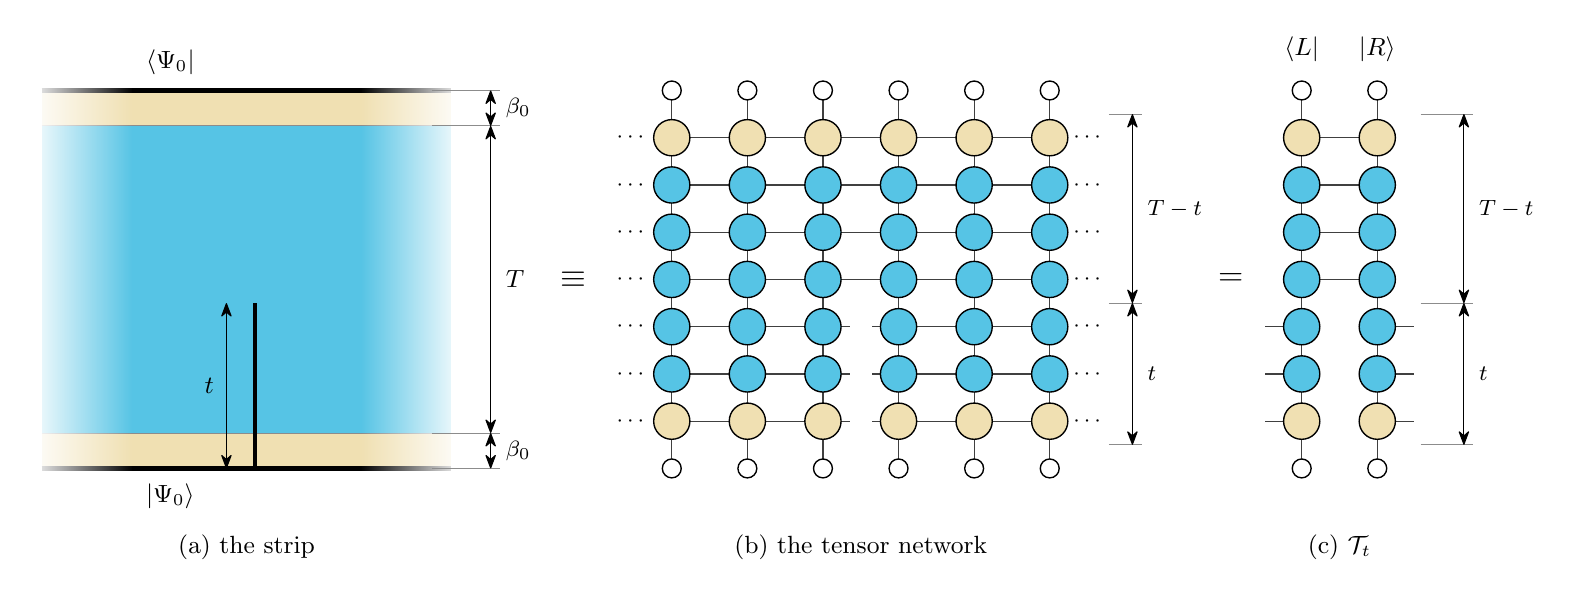
\begin{tikzpicture}[
    >={Stealth[round,length=2.0mm]},
    leg/.style={draw=black!75, line width=0.45pt},
    W/.style={circle, draw=black, fill=tnbulk, line width=0.5pt, minimum size=4.6mm, inner sep=0pt},
    B/.style={circle, draw=black, fill=tncool, line width=0.5pt, minimum size=4.6mm, inner sep=0pt},
    P/.style={circle, draw=black, fill=white, line width=0.5pt, minimum size=2.4mm, inner sep=0pt},
    cutline/.style={draw=black, line width=1.3pt},
    guide/.style={draw=black!45, line width=0.35pt},
    tag/.style={font=\small},
    idx/.style={font=\footnotesize},
  ]

  %% ================= panel (a): the strip, with the cut of height t =================
  \begin{scope}
    \def\SW{5.2}
    \def\YA{0} \def\YB{0.75} \def\YC{7.25} \def\YD{8}

    \fill[tncool] (0,{\YA*\DY}) rectangle (\SW,{\YB*\DY});
    \fill[tnbulk] (0,{\YB*\DY}) rectangle (\SW,{\YC*\DY});
    \fill[tncool] (0,{\YC*\DY}) rectangle (\SW,{\YD*\DY});
    \draw[black, line width=1.6pt] (0,{\YA*\DY}) -- (\SW,{\YA*\DY});
    \draw[black, line width=1.6pt] (0,{\YD*\DY}) -- (\SW,{\YD*\DY});
    \draw[guide] (0,{\YB*\DY}) -- (\SW,{\YB*\DY});
    \draw[guide] (0,{\YC*\DY}) -- (\SW,{\YC*\DY});

    \fill[white, path fading=east] (-0.18,{\YA*\DY-0.12}) rectangle (1.15,{\YD*\DY+0.12});
    \fill[white, path fading=west] ({\SW-1.15},{\YA*\DY-0.12}) rectangle ({\SW+0.18},{\YD*\DY+0.12});

    \node[tag, anchor=north west] at (1.2,{\YA*\DY-0.07}) {$\ket{\Psi_0}$};
    \node[tag, anchor=south west] at (1.2,{\YD*\DY+0.07}) {$\bra{\Psi_0}$};

    % the cut: a solid line from the bottom edge up to height t
    \draw[cutline] ({0.52*\SW},{\YA*\DY}) -- ({0.52*\SW},{\TCUT*\DY});
    \draw[<->] ({0.52*\SW-0.36},{\YA*\DY}) -- ({0.52*\SW-0.36},{\TCUT*\DY})
      node[midway, left=1pt, tag] {$t$};

    \def\XD{\SW+0.5}
    \foreach \y in {\YA,\YB,\YC,\YD} {
      \draw[guide] ({\SW-0.25},{\y*\DY}) -- ({\XD+0.12},{\y*\DY});
    }
    \draw[<->] ({\XD},{\YB*\DY}) -- ({\XD},{\YC*\DY}) node[midway, right=2pt, tag] {$T$};
    \draw[<->] ({\XD},{\YA*\DY}) -- ({\XD},{\YB*\DY}) node[midway, right=2pt, idx] {$\beta_0$};
    \draw[<->] ({\XD},{\YC*\DY}) -- ({\XD},{\YD*\DY}) node[midway, right=2pt, idx] {$\beta_0$};

    \node[tag] at ({\SW/2},-1.0) {(a) the strip};
  \end{scope}

  \node[font=\large] at (6.75,{4*\DY}) {$\equiv$};

  %% ================= panel (b): the tensor network, the cut removes the bonds =========
  \begin{scope}[xshift=8.0cm]
    \def\NX{5}

    \foreach \i in {0,...,\NX} { \draw[leg] (\i*\DX,0) -- (\i*\DX,{8*\DY}); }
    % every horizontal bond except those crossed by the cut
    \foreach \j in {1,...,7} {
      \foreach \i in {0,1,3,4} { \draw[leg] (\i*\DX,\j*\DY) -- ({(\i+1)*\DX},\j*\DY); }
    }
    \foreach \j in {4,...,7} { \draw[leg] ({2*\DX},\j*\DY) -- ({3*\DX},\j*\DY); }
    % below the cut there is no bond: each side keeps an open leg
    \foreach \j in {1,2,3} {
      \draw[leg] ({2*\DX},\j*\DY) -- ({2*\DX+0.34},\j*\DY);
      \draw[leg] ({3*\DX},\j*\DY) -- ({3*\DX-0.34},\j*\DY);
    }

    \foreach \i in {0,...,\NX} {
      \foreach \j in {1,7} { \node[B] at (\i*\DX,\j*\DY) {}; }
      \foreach \j in {2,...,6} { \node[W] at (\i*\DX,\j*\DY) {}; }
      \node[P] at (\i*\DX,0)       {};
      \node[P] at (\i*\DX,{8*\DY}) {};
    }
    \foreach \j in {1,...,7} {
      \node[idx] at (-0.5,\j*\DY)           {$\cdots$};
      \node[idx] at ({\NX*\DX+0.5},\j*\DY)  {$\cdots$};
    }

    % the two parts of the temporal chain
    \def\XB{\NX*\DX+1.05}
    \draw[guide] ({\NX*\DX+0.75},{0.5*\DY}) -- ({\XB+0.12},{0.5*\DY});
    \draw[guide] ({\NX*\DX+0.75},{\TCUT*\DY}) -- ({\XB+0.12},{\TCUT*\DY});
    \draw[guide] ({\NX*\DX+0.75},{7.5*\DY}) -- ({\XB+0.12},{7.5*\DY});
    \draw[<->] ({\XB},{0.5*\DY}) -- ({\XB},{\TCUT*\DY}) node[midway, right=2pt, idx] {$t$};
    \draw[<->] ({\XB},{\TCUT*\DY}) -- ({\XB},{7.5*\DY}) node[midway, right=2pt, idx] {$T-t$};

    \node[tag] at ({\NX*\DX/2},-1.0) {(b) the tensor network};
  \end{scope}

  %% ================= panel (c): the two halves contracted ============================
  \node[font=\large] at (15.1,{4*\DY}) {$=$};

  \begin{scope}[xshift=16.0cm]
    \def\CX{\DX}

    \draw[leg] (0,0) -- (0,{8*\DY});
    \draw[leg] (\CX,0) -- (\CX,{8*\DY});
    % above the cut the two columns are contracted with each other
    \foreach \j in {4,...,7} { \draw[leg] (0,\j*\DY) -- (\CX,\j*\DY); }
    % below it the open legs are redrawn pointing outwards
    \foreach \j in {1,2,3} {
      \draw[leg] (0,\j*\DY) -- (-0.46,\j*\DY);
      \draw[leg] (\CX,\j*\DY) -- ({\CX+0.46},\j*\DY);
    }

    \foreach \j in {1,7} { \node[B] at (0,\j*\DY) {}; \node[B] at (\CX,\j*\DY) {}; }
    \foreach \j in {2,...,6} { \node[W] at (0,\j*\DY) {}; \node[W] at (\CX,\j*\DY) {}; }
    \node[P] at (0,0) {};        \node[P] at (\CX,0) {};
    \node[P] at (0,{8*\DY}) {};  \node[P] at (\CX,{8*\DY}) {};

    \def\XC{\CX+1.1}
    \draw[guide] ({\CX+0.55},{0.5*\DY})   -- ({\XC+0.12},{0.5*\DY});
    \draw[guide] ({\CX+0.55},{\TCUT*\DY}) -- ({\XC+0.12},{\TCUT*\DY});
    \draw[guide] ({\CX+0.55},{7.5*\DY})   -- ({\XC+0.12},{7.5*\DY});
    \draw[<->] ({\XC},{0.5*\DY}) -- ({\XC},{\TCUT*\DY}) node[midway, right=2pt, idx] {$t$};
    \draw[<->] ({\XC},{\TCUT*\DY}) -- ({\XC},{7.5*\DY}) node[midway, right=2pt, idx] {$T-t$};

    \node[tag, anchor=south] at (0,{8*\DY+0.24})    {$\bra{L}$};
    \node[tag, anchor=south] at (\CX,{8*\DY+0.24})  {$\ket{R}$};

    \node[tag] at ({0.5*\CX},-1.0) {(c) $\mathcal{T}_t$};
  \end{scope}

\end{tikzpicture}
\end{document}
.
\documentclass[tikz,border=3pt]{standalone}
\usepackage{amsmath,amssymb,braket}
\usetikzlibrary{arrows.meta,fadings}

\newcommand{\DX}{0.96}
\newcommand{\DY}{0.60}
\newcommand{\TCUT}{3.5}      % height of the cut, in row units

\definecolor{tnbulk}{RGB}{86,196,229}
\definecolor{tncool}{RGB}{240,224,178}

\begin{document}
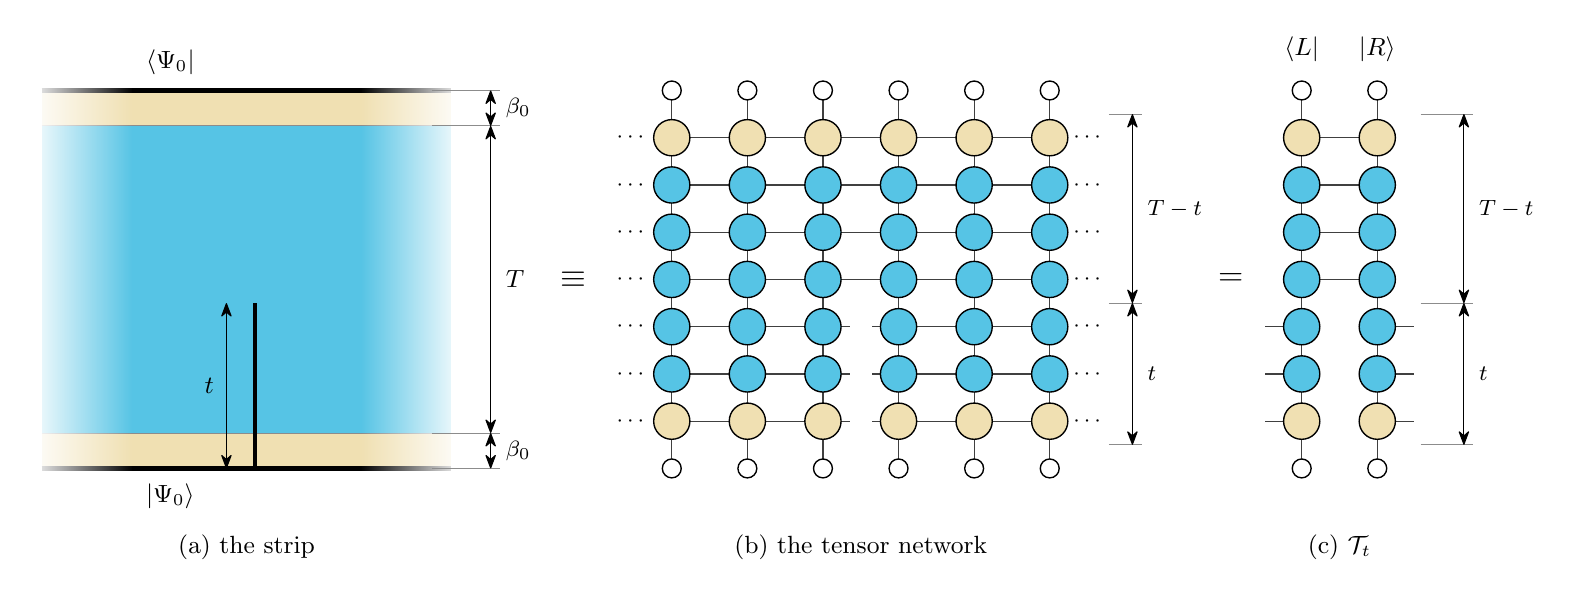
\begin{tikzpicture}[
    >={Stealth[round,length=2.0mm]},
    leg/.style={draw=black!75, line width=0.45pt},
    W/.style={circle, draw=black, fill=tnbulk, line width=0.5pt, minimum size=4.6mm, inner sep=0pt},
    B/.style={circle, draw=black, fill=tncool, line width=0.5pt, minimum size=4.6mm, inner sep=0pt},
    P/.style={circle, draw=black, fill=white, line width=0.5pt, minimum size=2.4mm, inner sep=0pt},
    cutline/.style={draw=black, line width=1.3pt},
    guide/.style={draw=black!45, line width=0.35pt},
    tag/.style={font=\small},
    idx/.style={font=\footnotesize},
  ]

  %% ================= panel (a): the strip, with the cut of height t =================
  \begin{scope}
    \def\SW{5.2}
    \def\YA{0} \def\YB{0.75} \def\YC{7.25} \def\YD{8}

    \fill[tncool] (0,{\YA*\DY}) rectangle (\SW,{\YB*\DY});
    \fill[tnbulk] (0,{\YB*\DY}) rectangle (\SW,{\YC*\DY});
    \fill[tncool] (0,{\YC*\DY}) rectangle (\SW,{\YD*\DY});
    \draw[black, line width=1.6pt] (0,{\YA*\DY}) -- (\SW,{\YA*\DY});
    \draw[black, line width=1.6pt] (0,{\YD*\DY}) -- (\SW,{\YD*\DY});
    \draw[guide] (0,{\YB*\DY}) -- (\SW,{\YB*\DY});
    \draw[guide] (0,{\YC*\DY}) -- (\SW,{\YC*\DY});

    \fill[white, path fading=east] (-0.18,{\YA*\DY-0.12}) rectangle (1.15,{\YD*\DY+0.12});
    \fill[white, path fading=west] ({\SW-1.15},{\YA*\DY-0.12}) rectangle ({\SW+0.18},{\YD*\DY+0.12});

    \node[tag, anchor=north west] at (1.2,{\YA*\DY-0.07}) {$\ket{\Psi_0}$};
    \node[tag, anchor=south west] at (1.2,{\YD*\DY+0.07}) {$\bra{\Psi_0}$};

    % the cut: a solid line from the bottom edge up to height t
    \draw[cutline] ({0.52*\SW},{\YA*\DY}) -- ({0.52*\SW},{\TCUT*\DY});
    \draw[<->] ({0.52*\SW-0.36},{\YA*\DY}) -- ({0.52*\SW-0.36},{\TCUT*\DY})
      node[midway, left=1pt, tag] {$t$};

    \def\XD{\SW+0.5}
    \foreach \y in {\YA,\YB,\YC,\YD} {
      \draw[guide] ({\SW-0.25},{\y*\DY}) -- ({\XD+0.12},{\y*\DY});
    }
    \draw[<->] ({\XD},{\YB*\DY}) -- ({\XD},{\YC*\DY}) node[midway, right=2pt, tag] {$T$};
    \draw[<->] ({\XD},{\YA*\DY}) -- ({\XD},{\YB*\DY}) node[midway, right=2pt, idx] {$\beta_0$};
    \draw[<->] ({\XD},{\YC*\DY}) -- ({\XD},{\YD*\DY}) node[midway, right=2pt, idx] {$\beta_0$};

    \node[tag] at ({\SW/2},-1.0) {(a) the strip};
  \end{scope}

  \node[font=\large] at (6.75,{4*\DY}) {$\equiv$};

  %% ================= panel (b): the tensor network, the cut removes the bonds =========
  \begin{scope}[xshift=8.0cm]
    \def\NX{5}

    \foreach \i in {0,...,\NX} { \draw[leg] (\i*\DX,0) -- (\i*\DX,{8*\DY}); }
    % every horizontal bond except those crossed by the cut
    \foreach \j in {1,...,7} {
      \foreach \i in {0,1,3,4} { \draw[leg] (\i*\DX,\j*\DY) -- ({(\i+1)*\DX},\j*\DY); }
    }
    \foreach \j in {4,...,7} { \draw[leg] ({2*\DX},\j*\DY) -- ({3*\DX},\j*\DY); }
    % below the cut there is no bond: each side keeps an open leg
    \foreach \j in {1,2,3} {
      \draw[leg] ({2*\DX},\j*\DY) -- ({2*\DX+0.34},\j*\DY);
      \draw[leg] ({3*\DX},\j*\DY) -- ({3*\DX-0.34},\j*\DY);
    }

    \foreach \i in {0,...,\NX} {
      \foreach \j in {1,7} { \node[B] at (\i*\DX,\j*\DY) {}; }
      \foreach \j in {2,...,6} { \node[W] at (\i*\DX,\j*\DY) {}; }
      \node[P] at (\i*\DX,0)       {};
      \node[P] at (\i*\DX,{8*\DY}) {};
    }
    \foreach \j in {1,...,7} {
      \node[idx] at (-0.5,\j*\DY)           {$\cdots$};
      \node[idx] at ({\NX*\DX+0.5},\j*\DY)  {$\cdots$};
    }

    % the two parts of the temporal chain
    \def\XB{\NX*\DX+1.05}
    \draw[guide] ({\NX*\DX+0.75},{0.5*\DY}) -- ({\XB+0.12},{0.5*\DY});
    \draw[guide] ({\NX*\DX+0.75},{\TCUT*\DY}) -- ({\XB+0.12},{\TCUT*\DY});
    \draw[guide] ({\NX*\DX+0.75},{7.5*\DY}) -- ({\XB+0.12},{7.5*\DY});
    \draw[<->] ({\XB},{0.5*\DY}) -- ({\XB},{\TCUT*\DY}) node[midway, right=2pt, idx] {$t$};
    \draw[<->] ({\XB},{\TCUT*\DY}) -- ({\XB},{7.5*\DY}) node[midway, right=2pt, idx] {$T-t$};

    \node[tag] at ({\NX*\DX/2},-1.0) {(b) the tensor network};
  \end{scope}

  %% ================= panel (c): the two halves contracted ============================
  \node[font=\large] at (15.1,{4*\DY}) {$=$};

  \begin{scope}[xshift=16.0cm]
    \def\CX{\DX}

    \draw[leg] (0,0) -- (0,{8*\DY});
    \draw[leg] (\CX,0) -- (\CX,{8*\DY});
    % above the cut the two columns are contracted with each other
    \foreach \j in {4,...,7} { \draw[leg] (0,\j*\DY) -- (\CX,\j*\DY); }
    % below it the open legs are redrawn pointing outwards
    \foreach \j in {1,2,3} {
      \draw[leg] (0,\j*\DY) -- (-0.46,\j*\DY);
      \draw[leg] (\CX,\j*\DY) -- ({\CX+0.46},\j*\DY);
    }

    \foreach \j in {1,7} { \node[B] at (0,\j*\DY) {}; \node[B] at (\CX,\j*\DY) {}; }
    \foreach \j in {2,...,6} { \node[W] at (0,\j*\DY) {}; \node[W] at (\CX,\j*\DY) {}; }
    \node[P] at (0,0) {};        \node[P] at (\CX,0) {};
    \node[P] at (0,{8*\DY}) {};  \node[P] at (\CX,{8*\DY}) {};

    \def\XC{\CX+1.1}
    \draw[guide] ({\CX+0.55},{0.5*\DY})   -- ({\XC+0.12},{0.5*\DY});
    \draw[guide] ({\CX+0.55},{\TCUT*\DY}) -- ({\XC+0.12},{\TCUT*\DY});
    \draw[guide] ({\CX+0.55},{7.5*\DY})   -- ({\XC+0.12},{7.5*\DY});
    \draw[<->] ({\XC},{0.5*\DY}) -- ({\XC},{\TCUT*\DY}) node[midway, right=2pt, idx] {$t$};
    \draw[<->] ({\XC},{\TCUT*\DY}) -- ({\XC},{7.5*\DY}) node[midway, right=2pt, idx] {$T-t$};

    \node[tag, anchor=south] at (0,{8*\DY+0.24})    {$\bra{L}$};
    \node[tag, anchor=south] at (\CX,{8*\DY+0.24})  {$\ket{R}$};

    \node[tag] at ({0.5*\CX},-1.0) {(c) $\mathcal{T}_t$};
  \end{scope}

\end{tikzpicture}
\end{document}
.
\documentclass[tikz,border=3pt]{standalone}
\usepackage{amsmath,amssymb,braket}
\usetikzlibrary{arrows.meta,fadings}

\newcommand{\DX}{0.96}
\newcommand{\DY}{0.60}
\newcommand{\TCUT}{3.5}      % height of the cut, in row units

\definecolor{tnbulk}{RGB}{86,196,229}
\definecolor{tncool}{RGB}{240,224,178}

\begin{document}
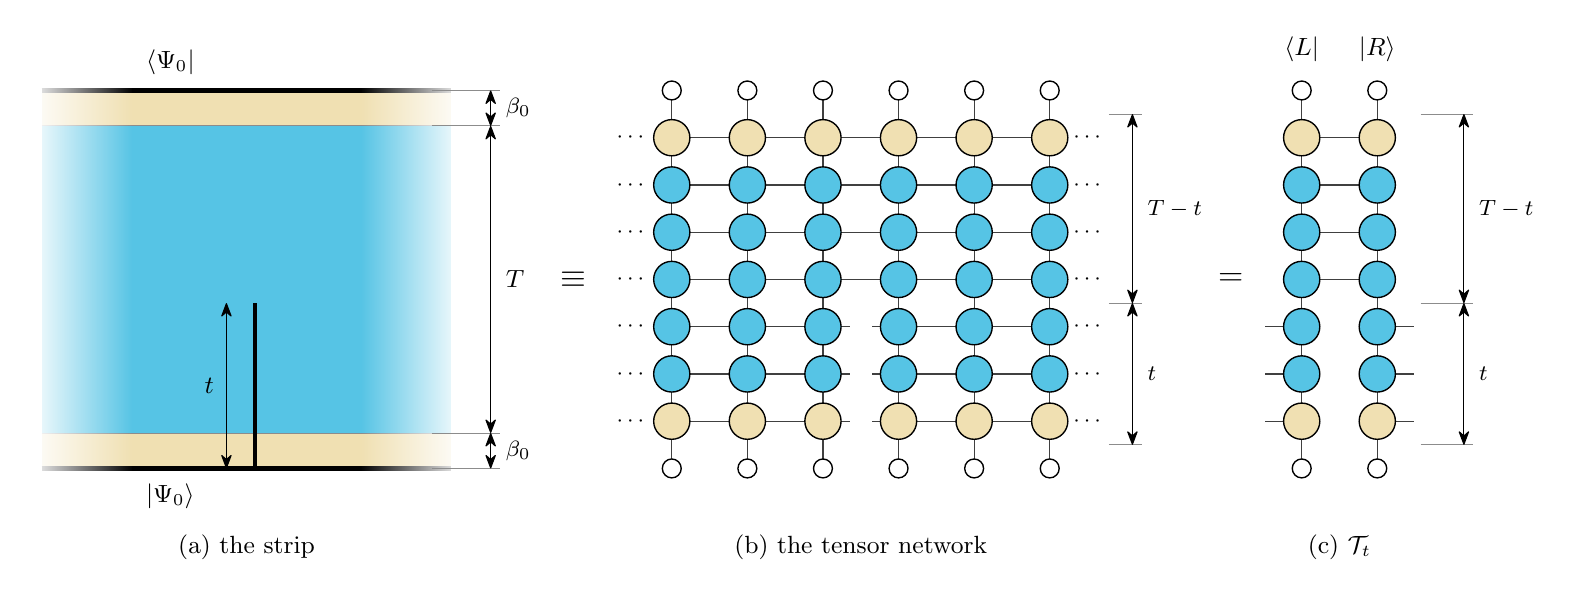
\begin{tikzpicture}[
    >={Stealth[round,length=2.0mm]},
    leg/.style={draw=black!75, line width=0.45pt},
    W/.style={circle, draw=black, fill=tnbulk, line width=0.5pt, minimum size=4.6mm, inner sep=0pt},
    B/.style={circle, draw=black, fill=tncool, line width=0.5pt, minimum size=4.6mm, inner sep=0pt},
    P/.style={circle, draw=black, fill=white, line width=0.5pt, minimum size=2.4mm, inner sep=0pt},
    cutline/.style={draw=black, line width=1.3pt},
    guide/.style={draw=black!45, line width=0.35pt},
    tag/.style={font=\small},
    idx/.style={font=\footnotesize},
  ]

  %% ================= panel (a): the strip, with the cut of height t =================
  \begin{scope}
    \def\SW{5.2}
    \def\YA{0} \def\YB{0.75} \def\YC{7.25} \def\YD{8}

    \fill[tncool] (0,{\YA*\DY}) rectangle (\SW,{\YB*\DY});
    \fill[tnbulk] (0,{\YB*\DY}) rectangle (\SW,{\YC*\DY});
    \fill[tncool] (0,{\YC*\DY}) rectangle (\SW,{\YD*\DY});
    \draw[black, line width=1.6pt] (0,{\YA*\DY}) -- (\SW,{\YA*\DY});
    \draw[black, line width=1.6pt] (0,{\YD*\DY}) -- (\SW,{\YD*\DY});
    \draw[guide] (0,{\YB*\DY}) -- (\SW,{\YB*\DY});
    \draw[guide] (0,{\YC*\DY}) -- (\SW,{\YC*\DY});

    \fill[white, path fading=east] (-0.18,{\YA*\DY-0.12}) rectangle (1.15,{\YD*\DY+0.12});
    \fill[white, path fading=west] ({\SW-1.15},{\YA*\DY-0.12}) rectangle ({\SW+0.18},{\YD*\DY+0.12});

    \node[tag, anchor=north west] at (1.2,{\YA*\DY-0.07}) {$\ket{\Psi_0}$};
    \node[tag, anchor=south west] at (1.2,{\YD*\DY+0.07}) {$\bra{\Psi_0}$};

    % the cut: a solid line from the bottom edge up to height t
    \draw[cutline] ({0.52*\SW},{\YA*\DY}) -- ({0.52*\SW},{\TCUT*\DY});
    \draw[<->] ({0.52*\SW-0.36},{\YA*\DY}) -- ({0.52*\SW-0.36},{\TCUT*\DY})
      node[midway, left=1pt, tag] {$t$};

    \def\XD{\SW+0.5}
    \foreach \y in {\YA,\YB,\YC,\YD} {
      \draw[guide] ({\SW-0.25},{\y*\DY}) -- ({\XD+0.12},{\y*\DY});
    }
    \draw[<->] ({\XD},{\YB*\DY}) -- ({\XD},{\YC*\DY}) node[midway, right=2pt, tag] {$T$};
    \draw[<->] ({\XD},{\YA*\DY}) -- ({\XD},{\YB*\DY}) node[midway, right=2pt, idx] {$\beta_0$};
    \draw[<->] ({\XD},{\YC*\DY}) -- ({\XD},{\YD*\DY}) node[midway, right=2pt, idx] {$\beta_0$};

    \node[tag] at ({\SW/2},-1.0) {(a) the strip};
  \end{scope}

  \node[font=\large] at (6.75,{4*\DY}) {$\equiv$};

  %% ================= panel (b): the tensor network, the cut removes the bonds =========
  \begin{scope}[xshift=8.0cm]
    \def\NX{5}

    \foreach \i in {0,...,\NX} { \draw[leg] (\i*\DX,0) -- (\i*\DX,{8*\DY}); }
    % every horizontal bond except those crossed by the cut
    \foreach \j in {1,...,7} {
      \foreach \i in {0,1,3,4} { \draw[leg] (\i*\DX,\j*\DY) -- ({(\i+1)*\DX},\j*\DY); }
    }
    \foreach \j in {4,...,7} { \draw[leg] ({2*\DX},\j*\DY) -- ({3*\DX},\j*\DY); }
    % below the cut there is no bond: each side keeps an open leg
    \foreach \j in {1,2,3} {
      \draw[leg] ({2*\DX},\j*\DY) -- ({2*\DX+0.34},\j*\DY);
      \draw[leg] ({3*\DX},\j*\DY) -- ({3*\DX-0.34},\j*\DY);
    }

    \foreach \i in {0,...,\NX} {
      \foreach \j in {1,7} { \node[B] at (\i*\DX,\j*\DY) {}; }
      \foreach \j in {2,...,6} { \node[W] at (\i*\DX,\j*\DY) {}; }
      \node[P] at (\i*\DX,0)       {};
      \node[P] at (\i*\DX,{8*\DY}) {};
    }
    \foreach \j in {1,...,7} {
      \node[idx] at (-0.5,\j*\DY)           {$\cdots$};
      \node[idx] at ({\NX*\DX+0.5},\j*\DY)  {$\cdots$};
    }

    % the two parts of the temporal chain
    \def\XB{\NX*\DX+1.05}
    \draw[guide] ({\NX*\DX+0.75},{0.5*\DY}) -- ({\XB+0.12},{0.5*\DY});
    \draw[guide] ({\NX*\DX+0.75},{\TCUT*\DY}) -- ({\XB+0.12},{\TCUT*\DY});
    \draw[guide] ({\NX*\DX+0.75},{7.5*\DY}) -- ({\XB+0.12},{7.5*\DY});
    \draw[<->] ({\XB},{0.5*\DY}) -- ({\XB},{\TCUT*\DY}) node[midway, right=2pt, idx] {$t$};
    \draw[<->] ({\XB},{\TCUT*\DY}) -- ({\XB},{7.5*\DY}) node[midway, right=2pt, idx] {$T-t$};

    \node[tag] at ({\NX*\DX/2},-1.0) {(b) the tensor network};
  \end{scope}

  %% ================= panel (c): the two halves contracted ============================
  \node[font=\large] at (15.1,{4*\DY}) {$=$};

  \begin{scope}[xshift=16.0cm]
    \def\CX{\DX}

    \draw[leg] (0,0) -- (0,{8*\DY});
    \draw[leg] (\CX,0) -- (\CX,{8*\DY});
    % above the cut the two columns are contracted with each other
    \foreach \j in {4,...,7} { \draw[leg] (0,\j*\DY) -- (\CX,\j*\DY); }
    % below it the open legs are redrawn pointing outwards
    \foreach \j in {1,2,3} {
      \draw[leg] (0,\j*\DY) -- (-0.46,\j*\DY);
      \draw[leg] (\CX,\j*\DY) -- ({\CX+0.46},\j*\DY);
    }

    \foreach \j in {1,7} { \node[B] at (0,\j*\DY) {}; \node[B] at (\CX,\j*\DY) {}; }
    \foreach \j in {2,...,6} { \node[W] at (0,\j*\DY) {}; \node[W] at (\CX,\j*\DY) {}; }
    \node[P] at (0,0) {};        \node[P] at (\CX,0) {};
    \node[P] at (0,{8*\DY}) {};  \node[P] at (\CX,{8*\DY}) {};

    \def\XC{\CX+1.1}
    \draw[guide] ({\CX+0.55},{0.5*\DY})   -- ({\XC+0.12},{0.5*\DY});
    \draw[guide] ({\CX+0.55},{\TCUT*\DY}) -- ({\XC+0.12},{\TCUT*\DY});
    \draw[guide] ({\CX+0.55},{7.5*\DY})   -- ({\XC+0.12},{7.5*\DY});
    \draw[<->] ({\XC},{0.5*\DY}) -- ({\XC},{\TCUT*\DY}) node[midway, right=2pt, idx] {$t$};
    \draw[<->] ({\XC},{\TCUT*\DY}) -- ({\XC},{7.5*\DY}) node[midway, right=2pt, idx] {$T-t$};

    \node[tag, anchor=south] at (0,{8*\DY+0.24})    {$\bra{L}$};
    \node[tag, anchor=south] at (\CX,{8*\DY+0.24})  {$\ket{R}$};

    \node[tag] at ({0.5*\CX},-1.0) {(c) $\mathcal{T}_t$};
  \end{scope}

\end{tikzpicture}
\end{document}
